Low-loss transverse mode question.
As always drawing out a schematic of the cavity helps:
\begin{figure}[H]
	\centering
	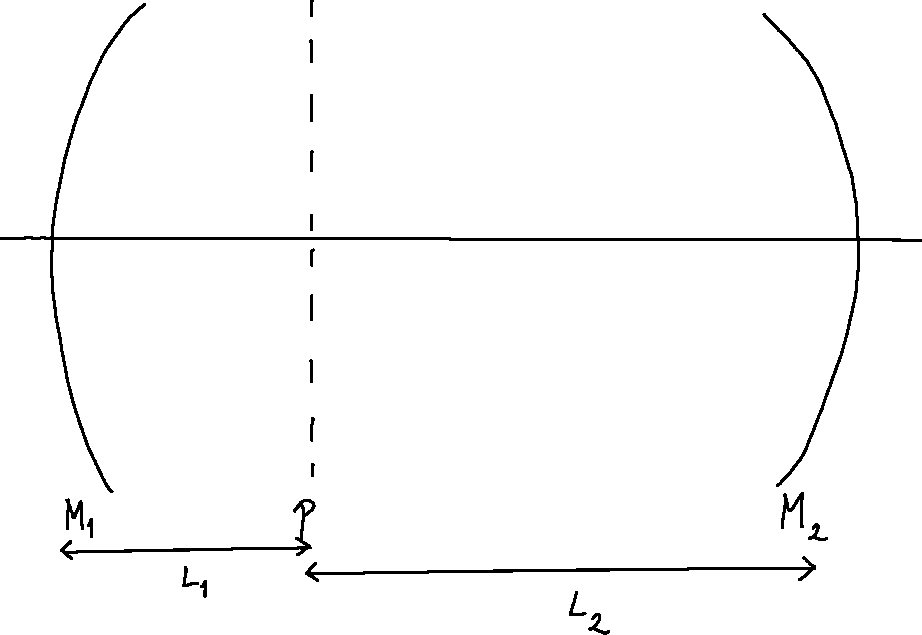
\includegraphics[width=.6\linewidth]{q2-cavity}
\end{figure}

\begin{parts}
	\part ABCD rule gives:
	\begin{equation*}
		q^\prime = \frac{Aq + B}{Cq + D}
	\end{equation*}
	
	And for a low-loss mode we have $q^\prime = q$:
	\begin{gather}
		Cq^{2} + Dq = Aq + B \notag \\
		Cq^{2} + (D-A)q - B = 0 \notag \\
		\Rightarrow q = \frac{(A-D) \pm \sqrt{(A-D)^{2} + 4BC}}{2C}
		\label{eqn:low-loss-q}
	\end{gather}
	
	We want $q$ to remain complex so the square-root term in \eqref{eqn:low-loss-q} must be negative:
	\begin{gather}
		(A-D)^{2} + 4\underbracket{BC}_{\substack{AD-BC=1 \\\Rightarrow BC=1+AD}} < 0 \notag \\[1ex]
		\Rightarrow (A+D)^{2} < 4 \notag \\
		\Rightarrow -2 < A+D < 2 \label{eqn:low-loss-cond}
	\end{gather}
	
	\part Ray transfer matrix for $\mathcal{P} \rightarrow M_1 \rightarrow \mathcal{P}$:
	\begin{align*}
		\begin{pmatrix}
			1 & L_1 \\
			0 & 1
		\end{pmatrix}
		\begin{pmatrix}
			1 & 0 \\[.5ex]
			-\dfrac{2}{R_1} & 1
		\end{pmatrix}
		\begin{pmatrix}
			1 & L_1 \\
			0 & 1
		\end{pmatrix}
		&= \begin{pmatrix}
			1 & L_1 \\
			0 & 1
		\end{pmatrix}
		\begin{pmatrix}
			1 & L_1 \\[1ex]
			-\dfrac{2}{R_1} & -\dfrac{2L_1}{R_1}+1
		\end{pmatrix} \\[1em]
		&= \begin{pmatrix}
			1-\dfrac{2L_1}{R_1} & 2L_1-\dfrac{2L_1^2}{R_1} \\[1em]
			-\dfrac{2}{R_1} & -\dfrac{2L_1}{R_1}+1
		\end{pmatrix}
	\end{align*}
	
	By symmetry, ray transfer matrix for $\mathcal{P} \rightarrow M_2 \rightarrow \mathcal{P}$:
	\begin{equation*}
		\begin{pmatrix}
			1-\dfrac{2L_2}{R_2} & 2L_2-\dfrac{2L_2^2}{R_2} \\[1em]
			-\dfrac{2}{R_2} & -\dfrac{2L_2}{R_2}+1
		\end{pmatrix}
	\end{equation*}
	
	Set $\mathcal{P}$ at $M_2$ gives $L_1=L$, $L_2=0$, thus the resultant matrix is:
	\begin{equation*}
		\begin{pmatrix}
			1 & 0 \\[1em]
			-\dfrac{2}{R_2} & 1
		\end{pmatrix}
		\begin{pmatrix}
			1-\dfrac{2L}{R_1} & 2L-\dfrac{2L^2}{R_1} \\[1em]
			-\dfrac{2}{R_1} & 1-\dfrac{2L}{R_1}
		\end{pmatrix}
		= \begin{pmatrix}
			1-\dfrac{2L}{R_1} & \ldots \\[1em]
			\ldots & -\dfrac{4L}{R_2}+\dfrac{4L^2}{R_1 R_2}+1-\dfrac{2L}{R_1}
		\end{pmatrix}
	\end{equation*}
	
	We then have $A+D$:
	\begin{align*}
		A+D &= 2-\frac{4L}{R_1}-\frac{4L}{R_2}+\frac{4L^2}{R_1 R_2} \\
		&= 4\rbracket{\frac{1}{2} - \frac{L}{R_1} - \frac{L}{R_2} \rbracket{1-\frac{L}{R_1}} } \\
		&= 4\sbracket{\rbracket{1-\frac{L}{R_1}} \rbracket{1-\frac{L}{R_2}} - \frac{1}{2}}
	\end{align*}
	
	Plugging this into \eqref{eqn:low-loss-cond} then gives:
	\begin{gather}
		-\frac{1}{2} < \rbracket{1-\frac{L}{R_1}} \rbracket{1-\frac{L}{R_2}} - \frac{1}{2} < \frac{1}{2} \notag \\
		0 < \underbracket{\rbracket{1-\frac{L}{R_1}}}_{g_1} \underbracket{\rbracket{1-\frac{L}{R_2}}}_{g_2} < 1 \label{eqn:low-loss-cond-sph}
	\end{gather}
	
	\part For a symmetric confocal cavity, $R_1=R_2=R$ and $L=R$, we then set $\mathcal{P}$ in the middle so $L_1=L_2=\diagfrac{L}{2}$.
	
	$\mathcal{P} \rightarrow M_1 \rightarrow \mathcal{P}$ gives:
	\begin{gather*}
		\begin{pmatrix}
			q^\prime \\ 1
		\end{pmatrix}
		= \mathcal{UF} \underbracket{\begin{pmatrix}
				1-\dfrac{L}{L} & L-\dfrac{L^2}{2L} \\[1em]
				-\dfrac{2}{L} & 1-\dfrac{L}{L}
		\end{pmatrix}}_{\begin{pmatrix}
				0 & \diagfrac{L}{2} \\
				-\diagfrac{2}{L} & 0
		\end{pmatrix}}
		\begin{pmatrix}
			q \\ 1
		\end{pmatrix} \\
		\Rightarrow q^\prime \equiv z_0^\prime - iz_R^\prime = \frac{\diagfrac{L}{2}}{-\diagfrac{2}{L}\times q} \textnormal{\hspace{1em}as per the definition of Gaussian beam} \\
		\Rightarrow z_0^\prime - iz_R^\prime = -\rbracket{ \frac{L}{2} }^2 \times \frac{1}{-iz_R} \\
		\Rightarrow z_0^\prime = 0 \textnormal{\hspace{1em}and\hspace{1em}} z_R z_R^\prime = \rbracket{ \frac{L}{2} }^2
	\end{gather*}
	
	Next we note that $\exp\rbracket{\dfrac{ik\rho^2}{2q}} = \exp\sbracket{\dfrac{ik\rho^2}{2}\rbracket{\dfrac{i}{z_R}}}=\exp\sbracket{-\dfrac{k\rho^2}{2z_R}}$ and thus the spot size $w \propto z_R$ ($\rho^2 = x^2 + y^2$ are the in-plane coordinates).
	
	Also we have $z_R^\prime = \dfrac{1}{z_R} \rbracket{\dfrac{L}{2}}^2$ and that $z_R^{\prime\prime} = z_R$ by the low-loss condition.
	
	We then have the sketch below:
	\begin{figure}[H]
		\centering
		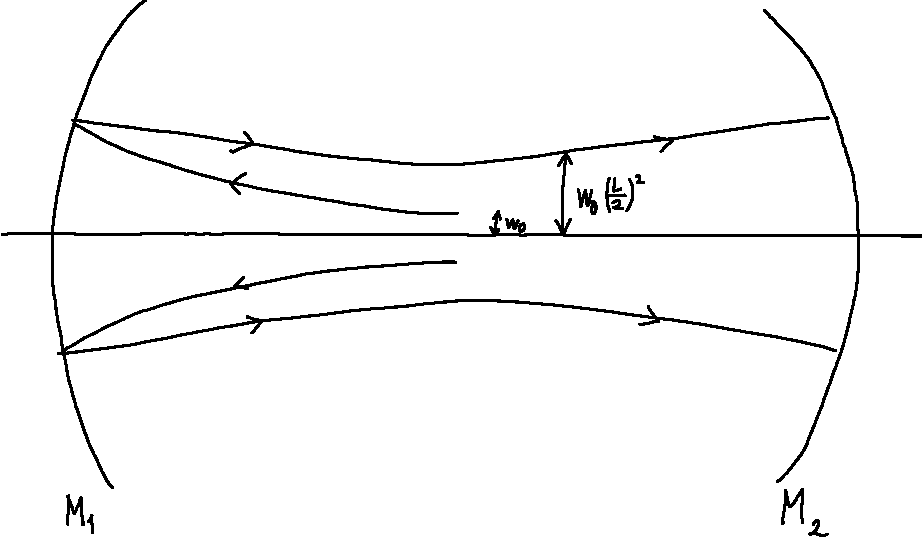
\includegraphics[width=.7\linewidth]{q2-waist}
	\end{figure}
	
	\part For the reflected beams to have the same spot size, we then need $z_R z_R^\prime = z_R^2 = (\diagfrac{L}{2})^2$:
	\begin{gather*}
		z_R = \frac{L}{2} \\
		\Rightarrow w^2 = \frac{2z_R}{k} \textnormal{\hspace{1em}at cavity centre} \\
		= \frac{2z_R}{\frac{2\pi}{\lambda}} \\
		= \frac{L\lambda}{2\pi}
	\end{gather*}
	
	At the mirror, we have:
	\begin{gather*}
		q = \frac{L}{2} - iz_R = \frac{L}{2}\rbracket{1-i} \\
		\Rightarrow \exp\sbracket{\frac{ik\rho^2}{2q}} = \exp\sbracket{\frac{ik\rho^2}{2}\times\frac{2}{L}\times\frac{1+i}{1^2+1^2}} \\
		= \exp\sbracket{-\frac{k\rho^2}{2L} + i\ldots}
	\end{gather*}
	So spot size $w^2 = \dfrac{2L}{k} = \dfrac{L\lambda}{\pi}$.
	
	Note that the $g_1 g_2$ factor in \eqref{eqn:low-loss-cond-sph} for a symmetric confocal cavity is borderline unstable, therefore in practice it can be undesirable to employ such cavity as slight disturbance can lead to high loss.
\end{parts}